\documentclass[../document.tex]{subfiles}
\documentclass{beamer}
\usepackage{amssymb,amsmath,amsthm}
\usepackage{graphicx}
\usepackage{tikz}
%\usetheme{Singapore}
\usetheme{Boadilla}
\usecolortheme{rose}

\usetikzlibrary{tikzmark}
\usepackage{colortbl}
\usepackage{graphicx}
\usepackage{pdfpages}
\tikzstyle{every picture}+=[remember picture,baseline]
\tikzstyle{every node}+=[inner sep=0pt,anchor=base,
minimum width=1.5cm,align=center,text depth=.25ex,outer sep=1.5pt]
\tikzstyle{every path}+=[thick, rounded corners]
%\setframetemplate{frametitle}[default][center]

%%%%%%%%%%%%%%%%%%%% VERY IMPORTANT 
%very useful way to add notes to Beamer
%\setbeameroption{show notes on second screen=right}
\setbeamertemplate{note page} 
{ 
	\insertslideintonotes{0.65} 
	\rule{\textwidth}{0.1pt} 
	\color{blue} \small
	\insertnote 
}

%%%%%%%%%%% for continuing slides enumeration
\newcounter{saveenumi}
\newcommand{\seti}{\setcounter{saveenumi}{\value{enumi}}}
\newcommand{\conti}{\setcounter{enumi}{\value{saveenumi}}}

\resetcounteronoverlays{saveenumi}



\begin{document}

\begin{frame}
	\begin{definition}[Synchronous distributed system]
		A distributed system comprising of processes is synchronous iff it has the following properties\footnotemark
		\begin{enumerate}
			\item<+-> There is a real-time physical clock which provides synchronization among multiple processes
			\item<.-> A known upper bound $\epsilon$ on processing delays
			\item<.-> A known upper bound $\delta$ on message transmission delays.
		\end{enumerate}
	\footnotetext[1]{\textit{"Reliable and Secure Distributed Programming"} A book by Rodrigues L. \& Cachin}
	\end{definition}

%%%%%%%%%%%%%%%%

\end{frame}
\begin{frame}{Asynchronous systems $\rightarrow$ Lamport's Time clocks revisted}
	\small
	\begin{definition}[Asynchronous system\footnotemark]
		In such systems, there is no time assumptions about processes. That is, we do not have \textbf{physical clock}. Instead \textbf{Time} is defined with respect to communication and measured by a \textit{Logical clock}.  
	\end{definition}
	\uncover <2-> {Here is Lamport's Algorithm for finding something has "happened before" something else.}
	\footnotetext[1]{\textit{"Reliable and Secure Distributed Programming"} A book by Rodrigues L. \& Cachin}
\end{frame}

%%%%%%%%%%%%%

\begin{frame}{A brief description of Lamport's Algorithm for Time clocks}
	\begin{enumerate}
		\item <+-> Each process $p$ keeps an ineger called \textit{logical clock $l_p$} initially 0.
		\item <+-> Whenver an event occurs at Node $p$, the logical clock $l_p$ is incremented by one unit.
		\item <+-> When a process \textbf{sends a message,} it adds a timestamp to the message with the value of its logical clock at the moment the message is sent. The timestamp of an event $e$ is denoted by $t(e)$.
		\item<+-> When a Node $p$ receives a message $m$ with timestamp $t_m$, Node $p$ increments its logical clock in the following way: $l_p := \max\{l_p, t_m\} + 1$
	\end{enumerate}
\end{frame}

%%%%%%%%%%%%%%

\begin{frame}{A brief description of Lamport's Algorithm for Time clocks \textit{cont.}}
	\begin{itemize}
		\item <+-> now that we have a mechanism for time in asynchronous world, let us define the \textit{happened before} relation
	\end{itemize}
\small
		\uncover <+-> { \begin{definition}[Happened before relation $e_1\rightarrow e_2$]
				
			For event $e_1$ and $e_2$ we say "$e_1$ \textit{has happened before} $e_2$" ($e_1\rightarrow e_2$) if $e_1$ and $e_2$ have the following conditions:
			\begin{enumerate}
				\item $e_1$ and $e_2$ occurred at the \textbf{same process p} and $e_1$ occurred before $e_2$ (i.e. $t(e_2) = t(e_1) + 1$) 	\note<.->{- event is something such as sending or receiving message. \newline}
				\item $e_1$ corresponds to the transmission of a message $\pmb{m}$ at process $p$ and $e_2$ to the reception of $m$ at process $q$.
				\item $\rightarrow$ be transitive. 	\note<.->{- there exists some event $e'$ s.t. $e_1\rightarrow e'$ and $e'\rightarrow e_2$}
			\end{enumerate}
			\end{definition}}
	\footnotetext[1]{\textit{"Reliable and Secure Distributed Programming"} A book by Rodrigues L. \& Cachin}
\end{frame}


\begin{frame}[t]{A brief description of Lamport's Algorithm for Time clocks \textit{cont.}}

	\uncover<+->{The above definition implies that if $e_1 \rightarrow e_2\implies t(e_1) < t(e_2)$\\}
	\uncover<+->{
		\begin{tikzpicture}[remember picture,overlay]
			\node[above=6pt,xscale=1.7] at(current 	page.south) { %for relative positioning, we use \node [left=1cm or right or below or above] 
				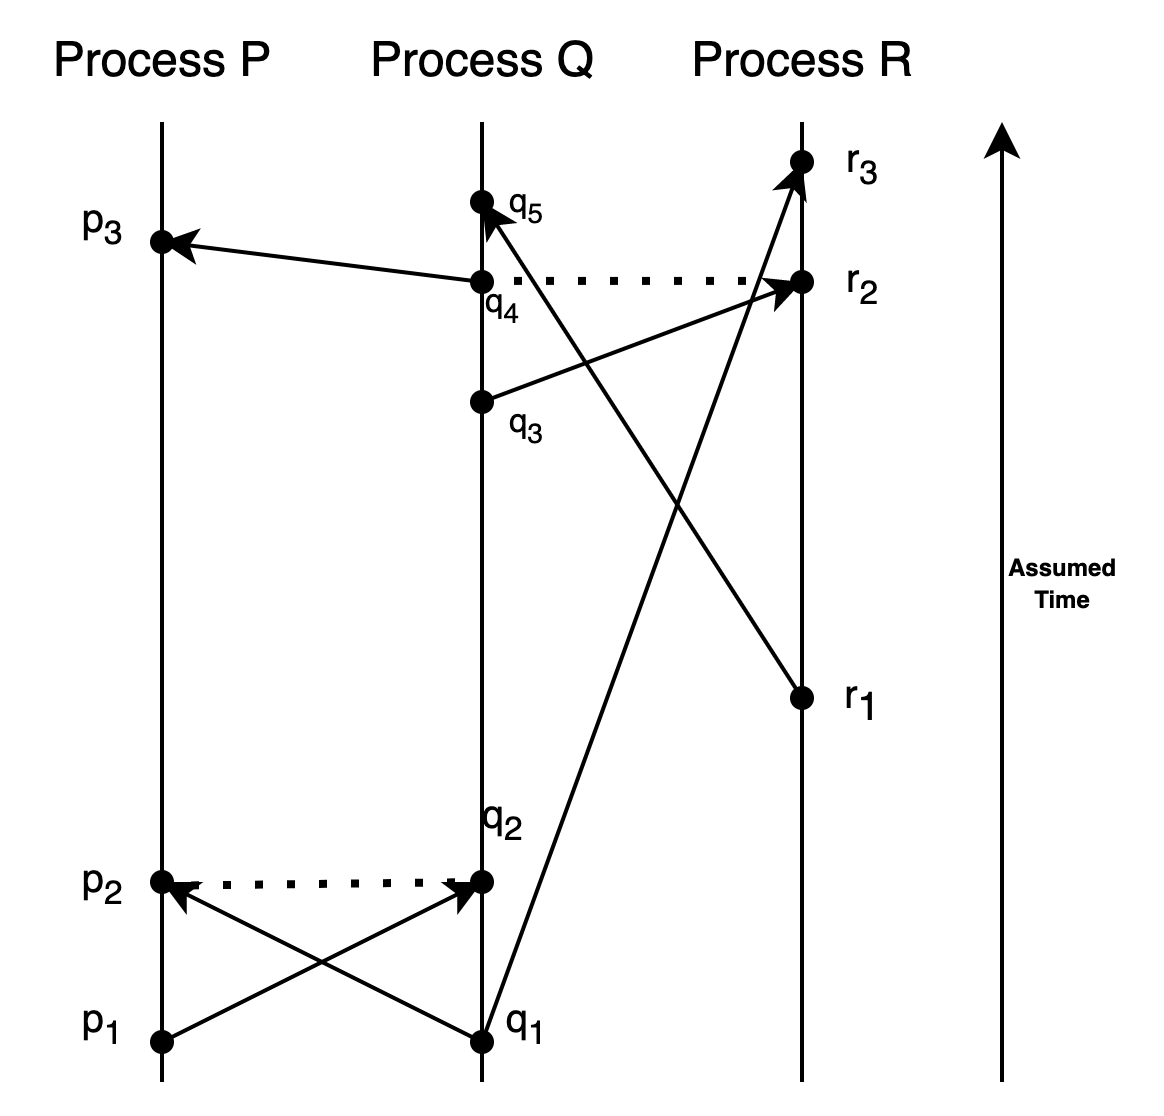
\includegraphics[width=0.6\textwidth]{../fig4.png}	
			};
	\end{tikzpicture}
}

\end{frame}
%%%%%%%%%%

\begin{frame}{Practical Byzantine Fault Tolerance (PBFT)}
This Algorithm describes the implementation of a \textbf{Byzantine-fault-tolerant disributed file system.}\\
Assumptions:\\
\begin{enumerate}
	\footnotesize
	\item <+-> We have a \textbf{asynchronous distributed system} $\implies$ network may have: \textbf{Delays, failure to deliver messages; duplicate them, delivery out of order}
	\item<+-> For Byzantine assumption (nodes behaving arbitrarily): Independent node failures $\implies$ each node runs service code \textbf{independently}, have different root password and a different admin.
	\item<+-> Use cryptographic techniques to prevent spoofing and to detect corrupted messages $\rightarrow$ messages have \textit{public key signatures}, message authentication codes.
	 \item<+-> A strong adversary coordinates faulty nodes, delay communication and delay correct nodes
	 \item<.-> The adversary cannot violate cryptographic techniques used by nodes. \note<.->{For example, the adversary cannot produce a valid signature of a non-faulty node, compute the information summarized by a digest from the digest, or find two messages with the same digest. The cryptographic techniques we use are thought to have these properties}
\end{enumerate}

\end{frame}

%%%%%%%%%%%%%%%%

\begin{frame}{Practical Byzantine Fault Tolerance (PBFT)}
	Properties: \\
	\begin{enumerate}
		\item <+-> The algorithm used to implement any \textbf{replicated service} with \textit{state} and \textit{some operations,} including but not limited to \textit{read and writes on replicas}
		\item<+-> There are some \textbf{faulty} and \textbf{non-faulty clients(requesting to invoke operations)} and \textbf{replicas} (we have \textbf{$f$} faulty replicas and $n=3f+1$ number of all replicas))\note<+->{Faulty clients are dealt with by \textbf{strong authentication}}
		\item<+-> The Algorithm both provides \textbf{safety} and \textbf{liveness}
		\begin{enumerate}
			\item<+-> \textbf{Safety (Accuracy):} replicated service satisfies linearizability. \note<.->{- It behaves like a centralized implementation that executes operations \textbf{atomically} one at a time.\\}
			\item<+-> \textbf{Liveness (Completeness):}  Clients eventually receive replies to their requests, provided at most $\lfloor \frac{n-1}{3}\rfloor$ are faulty and \underline{$delay(t)$} does not grow faster than $t$ indefinitely. \note<.->{-$delay(t)$ is the time between the moment when a message is sent for the first time and the moment when it is received by its destination (assuming the sender keeps retransmitting the message until it is received)}
			\seti
		\end{enumerate}
	\end{enumerate}
\end{frame}

%%%%%%%%%%%%%%%%%%%%

\begin{frame}[<+->]
	\begin{enumerate}
		\conti
		\item<+-> Algorithm does not rely on \textbf{synchrony} to provide \textbf{safety}
		\item<+-> However, \textbf{It must} rely on synchrony to provide \textbf{liveness} $\rightarrow$ \textbf{FLP's impossibility}
		\item<+-> The algorithm uses a 3-phase commit protocol: Pre-prepare, prepare, commit
		\seti
	\end{enumerate}
\end{frame}

\begin{frame}{PBFT Algorithm}
	\begin{itemize}
		\item <+-> There is a primary replica in each request of a client c. 
		\item<+-> Replicas move through a seccession of configurations called \textbf{views}.
		\item <+-> in a view, one replica is the primary and others are backups. 
	\end{itemize}

\end{frame}

\begin{frame}{PBFT Alg. Cont.}
	\uncover<+->{A very brief description of the Algorithm:}
	\begin{itemize}
		\item<+-> A client sends a request to invoke a service operation to the primary replica
		\item<+-> The client's request message is of the form $<REQUEST, o, t, c>_{\sigma_{c}}$ \note<.->{\small c is client, o is the operation needed, timestamp t is used to ensure \textbf{exactly once } semantics for the execution of client requests.}
		\item<+-> The primary multicasts the request to the backups
		\item<+-> Replicas execute the request and send a reply to the client
		\item<+-> The client waits for $f+1$ replies from different replicas with the same result; this the result of the operation.
		\item<+-> The replica's reply is of the form $<REQUEST, \nu, t, c, i, r>_{\sigma_{i}}$ \note<.->{\small v is the current view number, t is the timestamp of the corresponding request, i is the replica number, and r is the result of executing the requested operation}
	\end{itemize}
\end{frame}
%%%%%%%%%

\begin{frame}{PBFT Alg. Cont.}
\begin{itemize}
	\item<+-> The client waits for $f+1$ replies with valid signatures from different replicas, and with the same $t$ and $r$, before accepting the result $r$
	\item<+-> If client doesn't receive replies soon, it broadcasts the request to all replicas.
	\item<+-> If the request has already been processed, the replicas simply re-send the reply;
	\item<+-> otherwise, if the replica is not the primary, it relays the request to the primary. 
	\item<+-> If the primary doesn't multicast the request to the group, it will eventually be suspected to be faulty by enough replicas to cause a view change.
	\item<+-> \textbf{The algorithm is proved to be Only 3\% slower than non-replicated implementation of NFS}
\end{itemize}

\end{frame}
\end{document}